\chapter{Kompilacja systemu wbudowanego}
\label{ch:kompilacja}

Rozdział ten opisuje proces dostosowania oraz budowy dedykowanego obrazu jądra systemu operacyjnego Linux i~docelowego systemu plików (ang. \textit{rootfs}). Z~uwagi na konieczność maksymalnej optymalizacji, pozbycia się zbędnego oprogramowania (tzw. \textit{bloatware}) oraz specyfikę rozwiązań czasu rzeczywistego, w~projekcie zrezygnowano z~wykorzystania standardowych, desktopowych dystrybucji (takich jak Ubuntu). Zamiast tego zdecydowano się na wygenerowanie środowiska operacyjnego ściśle dopasowanego do założeń sprzętowych.

\section{System plików Yocto Project}
Aby stworzyć maksymalnie zoptymalizowane, lekkie i~wolne od narzutu zbędnych usług środowisko uruchomieniowe, zastosowano system budowania Yocto Project. Obecnie wykorzystano fundamentalną dystrybucję referencyjną Poky, co pozwoliło na znaczne zmniejszenie rozmiaru partycji \textit{rootfs} i~zagwarantowało wysoką wydajność systemu w~kontekście aplikacji czasu rzeczywistego (RT, ang. \textit{Real-Time}). Rozwiązanie to stanowi stabilną bazę i~pozostawia ogromne pole do dalszego, modułowego rozwoju (np. poprzez dodawanie nowych warstw i~pakietów) w~kolejnych etapach życia projektu.

\section{Struktura repozytorium i~źródła jądra systemu}
Płytka ewaluacyjna Terasic DE25 Nano oparta o~układ Intel Agilex 5 stanowi wysoce specyficzną platformę sprzętową (ang. \textit{custom hardware}), dla której standardowe jądro (ang. \textit{vanilla kernel}) nie zawiera wystarczającego wsparcia. Aby zagwarantować pełną kompatybilność sprzętową, konieczne było wykorzystanie jądra dostarczanego bezpośrednio przez producenta.

W~tym celu wykonano rozgałęzienie (ang. \textit{fork}) oficjalnego repozytorium \texttt{linux-socfpga} firmy Terasic. Repozytorium to zostało zintegrowane z~głównym katalogiem roboczym całego projektu przy wykorzystaniu mechanizmu submodułów (ang. \textit{Git submodules}). Zastosowanie takiego rozwiązania pozwala na wygodne śledzenie zmian w~kodzie producenta, a~jednocześnie umożliwia pełną kontrolę nad własnymi modyfikacjami, na które złożyła się m.in. implementacja łaty czasu rzeczywistego \texttt{PREEMPT\_RT} oraz włączenie wsparcia dla wymaganych komponentów sprzętowych.

\section{Konfiguracja jądra Linux i~środowisko kompilacji}
Proces konfiguracji jądra (Kconfig) został przeprowadzony w~celu włączenia obsługi dedykowanych mechanizmów sprzętowych. Korzystając z~interfejsu \texttt{menuconfig}, do głównego drzewa dodano między innymi obsługę sterownika układu AMC6821, który pełni na płytce funkcję sprzętowego monitora parametrów oraz inteligentnego kontrolera wentylatora. Wynikowa konfiguracja została zapisana do pliku \texttt{defconfig}, gwarantując powtarzalność procesu kompilacji.

Proces budowania obrazu \texttt{Image} jest realizowany przy pomocy narzędzi do kompilacji skrośnej (ang. \textit{cross-compilation toolchain}) dla architektury ARM64 (\texttt{aarch64-linux-gnu-gcc}). Aby zapewnić spójność środowiska budowania, główne zmienne systemowe definiujące ścieżki i~narzędzia ujęto bezpośrednio w~głównym pliku \texttt{Makefile} projektu:

\begin{lstlisting}[language=make, caption={Fragment pliku Makefile definujący zmienne dla kompilacji skrośnej}, label={lst:makefile_cross}]
export ARCH ?= arm64
export CROSS_COMPILE ?= aarch64-linux-gnu-

export KDIR := $(CURDIR)/linux-source
export INCLUDE_DTS := $(KDIR)/arch/arm64/boot/dts/intel
\end{lstlisting}

Wyeksportowanie zmiennej \texttt{KDIR} wskazującej na zmodyfikowane i~skompilowane źródła jądra jest kluczowe dla dalszych etapów projektu. Pozwala to na bezpośrednie i~bezkonfliktowe budowanie własnych, zewnętrznych modułów jądra (sterowników \texttt{.ko}) oraz kompilację drzewa urządzeń (ang. \textit{Device Tree}, pliki \texttt{.dtb}), gwarantując, że zostaną one skonsolidowane z~dokładnie tym samym wydaniem jądra, które zostanie uruchomione na platformie docelowej.

\begin{figure}[htbp]
    \centering
    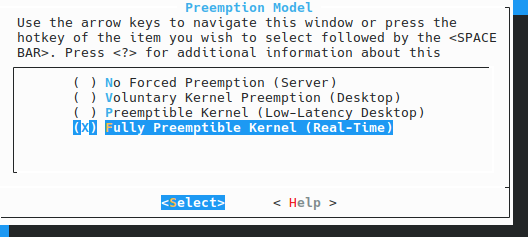
\includegraphics[width=0.75\textwidth]{rysunki/kconfig.png} % Dostosuj ścieżkę do swojego pliku
    \caption{Widok interfejsu narzędzia \texttt{menuconfig} przedstawiający aktywację w~pełni wywłaszczalnego jądra czasu rzeczywistego (łata PREEMPT\_RT).}
    \label{fig:kconfig_rt}
\end{figure}